\documentclass[11pt, a4paper]{report}

\usepackage[english]{babel}
\usepackage[utf8x]{inputenc}
\usepackage{amsmath}
\usepackage[normalem]{ulem}
\useunder{\uline}{\ul}{}
\usepackage{adjustbox}
\usepackage{float}
\usepackage[colorinlistoftodos]{todonotes}

\usepackage{fullpage}
% A more tightly packed list than the standard
% \enumerate{itemize} append * after enumeration type
\usepackage{mdwlist}
% Multi-page tables + accompanying header and footer comments
\usepackage{longtable}

% Vertical table headers, not sure what does what. graphicx is
% multi-purpose and does a lot of other stuff like including images
\usepackage{array,graphicx}
\usepackage{booktabs}

% Lossless .png format expected for figures
\DeclareGraphicsExtensions{.png}

% \verbatiminput command (\begin{verbatim} is standard lib)
\usepackage{verbatim}
% Allows for verbatiminput of files AND breaks lines that are too long
% for the page to fit
\usepackage{listings}

\newcommand*\rot{\rotatebox{90}}

\title{Modeling a Mobile Social Media Application}
\author{Matthew Flickner \\ Loyola Marymount University\\ CMSI486}

% Allow commands
\providecommand\phantomsection{}



\begin{document}

%---    Title page    ---%
\clearpage
\phantomsection
\addcontentsline{toc}{chapter}{%
    \protect\numberline{I}Title Page}
\maketitle


\tableofcontents
\newpage

\chapter{Description of Enterprise}
Matthew Flickner wants build an application to help people manage their responsibilities within a group of friends. He wants to use it to make tasks like household chores easier and more convenient while holding each person accountable for their responsibilities. He needs a reliable database to support the application and store application and user data. Matt needs to store user information for login. There is also a need for keeping track of what users are in what groups and whom the users are friends with. He also needs to track what tasks are in what groups and which user is responsible for completing a given task. Tasks can also have deadlines for when they need to be completed by and users can get points for completing tasks. A user gets one point for completing a task if they are the responsible party and 2 points if they volunteer to complete the task. A user can pay 5 points to get out of doing a particular task. Each user has a their own points within a given group. When the task is completed, a new person responsible is assigned or the task is closed.
\\
The following is an initial list of questions that the database for Matt’s application will need to answer:
\begin{itemize}
\item What groups is user John Smith a member of?
\item What tasks are in the group “House Stuff”?
\item Who is the person responsible for completing the task, “Empty the Dishwasher,” in the group, “House Stuff”?
\item Is the “Wipe off the counters” a one-time task or a repeating task?
\item How many points does user Logan Couture have allocated for completing the task “Take out the trash”?
\item Does user Patrick Marleau have less or more points in the task “Take out the trash” than Logan Couture?
\item Is Marshall Shady a friend of George Clooney?
\item Who is in the group “Stuff to Do”?
\item When does task “Clean Sink” in the group “Kitchen” need to be completed by?
\end{itemize}

\chapter{Definition of the Environment}
\section{Input and Report Forms}

\subsection*{User Creation Form}
\begin{itemize}
\item First Name
\item Last Name
\item Username
\item Password
\item Email Address
\end{itemize}

\subsection*{User Login View}
\begin{itemize}
\item Username
\item Password
\end{itemize}

\subsection*{UserGroup Creation Form}
\begin{itemize}
\item GroupId
\item UserId
\item isGroupAdmin
\end{itemize}

\subsection*{Group Creation View}
\begin{itemize}
\item Group Name
\item Group Members (usernames)
\end{itemize}

\subsection*{Leave Group View}
\begin{itemize}
\item Group Id
\item Group Members
\item User Group
\end{itemize}

\subsection*{Group Deletion View}
\begin{itemize}
\item Group Name
\item Group Members (usernames)
\item Group Tasks
\item Group Id
\end{itemize}

\subsection*{Task Creation Form}
\begin{itemize}
\item Task Name
\item Task Members
\item Group That Task Belongs To
\item Person Responsible For Completion
\end{itemize}

\subsection*{Task Completion View}
\begin{itemize}
\item Task Name
\item Task Members
\item Group That Task Belongs To
\item Person Who Completes Task
\item	Person Responsible for Next completion
\item Points For Task
\end{itemize}

\subsection*{Volunteer for Task Completion View}
\begin{itemize}
\item Task Name
\item Task Members
\item Group That Task Belongs To
\item Person Responsible For Completion
\end{itemize}

\subsection*{Opt-Out of Task View}
\begin{itemize}
\item Task Id
\item User's Point in Task
\item New Person Responsible For Completion
\end{itemize}


\section{Assumptions}
\begin{itemize}
\item Group Members and Task Members are not always the same list of people
\item Person Responsible For Completion is one person in Task Members
\item Usernames are unique
\item Usernames contain must be between 4-16 characters and be composed only of letters and numbers
\item Only one account is allowed per email address
\item Passwords must be at least 6 characters
\item 1 Point is awarded for the completion of the task when the user is the Person Responsible For Completion
\item 2 Points are awarded for the completion of the task when the user volunteers to be the Person Responsible For Completion.
\end{itemize}

\section{User-oriented data dictionary}
\begin{table}[H]
\centering
\begin{tabular}{| l | l |}
Datum & Information Definition \\\hline

user\_id & The unique id given to a user\\
username & The unique identifier of a user\\
first\_name & The first name of the user\\
last\_name & The last name of the user\\
password & The password of the user\\
email & The email address of the user\\

user\_group\_id & The unique id given to a user within a group\\
is\_group\_admin & Boolean that tells whether a user is a admin of their group\\

group\_id & The unique id given to a user\\
group\_name & The name of a group\\

task\_id & The unique id of a given task\\
task\_name & The name of the task\\

user\_group\_task\_id & The unique id of a user in a group for a particular task.\\
points & The number of points a user has for a given task within a group.\\
is\_desi & Boolean that tells whether or not a person is responsible for a given task.\\

task\_action\_id & The unique id of an action a user performs in a group for a specific task. \\
completed\_date & The date of the last time a task was completed.\\
volunteered\_completion & The date task's volunteer completed.\\
opt\_out & The date of the last time a user opted out of a given task in a given group.\\

friendship\_id & The unique id of a friendship between two users\\


\end{tabular}
\end{table}

\section*{Cross-reference table}

\begin{longtable}{|l|l|l|l|l|l|l|l|l|l|l|}

\hline
\multicolumn{1}{|c|}{Datum} &
\multicolumn{10}{c|}{Form or Screen} \\[1ex]

\hline
&   % empty label block
\rot{User Creation Form} &
\rot{User Login View} &
\rot{Group Creation View} &
\rot{Leave Group View} &
\rot{Group Deletion View} &
\rot{Task Creation Form} &
\rot{Task Completion View} &
\rot{Volunteer for Task Completion View} &
\rot{Opt-Out of Task View} &
\rot{Add Friend Form} \\
\hline

user\_id               & x  & x  &   & x  &   &   &  &  &  & x  \\ \hline
username            & x  & x  &  x &   &   &   &  &  &   &   \\ \hline
first\_name          &  x &   &   &   &   &   &   &   &   &   \\ \hline
last\_name           &  x &   &   &   &   &   &  & x &   &   \\ \hline
password             &  x & x  &   &   &   &   &  &  &   &   \\ \hline
email\_address    &  x &  x &   &   &   &   &   &  &   &   \\ \hline

group\_id              &   &   & x  & x  & x  &   &   &   &   &   \\ \hline
group\_name        &   &   & x  &   &   &   &   &   &   &   \\ \hline

user\_group\_id    &   &   & x & x & x &  &   &   &  &   \\ \hline
is\_group\_admin  &   &   &   & x & x &  &   &   &  &   \\ \hline

task\_id                 &   &   &   &   &   & x  & x  & x  & x &   \\ \hline
task\_name           &   &   &   &  &   &  x  &  &   &   &   \\ \hline


user\_group\_task\_id   &   &   &   &   &   & x  &  x &  x & x &   \\ \hline
points                            &   &   &   &   &   & x  & x  & x  & x  &  \\ \hline
is\_desi                         &   &   &   &   &   &  x &  x & x  & x  &  \\ \hline

friendship\_id     &   &   &   &   &   &   &   &   &   & x   \\ \hline

task\_action\_id &   &   &   &   &   &   & x  & x & x & \\ \hline
date\_completed &   &   &   &   &  &   &  x  &   &   & \\ \hline
volunteer\_completed &   &   &   &   &  &   &   & x  &   & \\ \hline
opt\_out &   &   &   &   &  &   &   &   & x  & \\ \hline



\end{longtable}



\chapter{Enterprise Database Design}
\section{Logical Model of the Enterprise}

\subsection{List of Entities and Attributes}
\begin{table}[H]
\centering
\begin{tabular}{|l|l|}
\hline
{\ul \textbf{Entity}} & {\ul \textbf{Attributes}}                                                                                                                              \\ \hline
user                  & \begin{tabular}[c]{@{}l@{}}user\_id(PK), username, first\_name, last\_name, password, email\_address\end{tabular} \\ \hline
friend                & \begin{tabular}[c]{@{}l@{}}friend\_id(PK), user\_id(FK) \end{tabular} \\ \hline
group                & \begin{tabular}[c]{@{}l@{}}group\_id(PK), group\_name, \end{tabular}                             \\ \hline
task                  & \begin{tabular}[c]{@{}l@{}}task\_id(PK), group\_id, desi(FK), desi\_index\end{tabular}             \\ \hline
task\_action       & \begin{tabular}[c]{@{}l@{}}task\_action\_id(PK), user\_group\_task\_id(FK) \end{tabular} \\ \hline
completion      & \begin{tabular}[c]{@{}l@{}}task\_action\_id(PK, FK), completed\_date \end{tabular} \\ \hline
volunteer\_completion & \begin{tabular}[c]{@{}l@{}}task\_action\_id(PK, FK), volunteer\_completed \end{tabular} \\ \hline
opt\_out & \begin{tabular}[c]{@{}l@{}}task\_action\_id(PK, FK), opt\_out\_date \end{tabular} \\ \hline


\end{tabular}
\end{table}

\subsection{List of Relationships and Attributes}
\begin{table}[H]
\centering
\begin{tabular}{|l|l|}
\hline
{\ul \textbf{Relationship}} & {\ul \textbf{Attributes}} \\ \hline
user\_group & user\_group\_id(PK), group\_id(FK), user\_id(FK), is\_group\_admin \\ \hline
user\_group\_task & \begin{tabular}[c]{@{}l@{}}user\_group\_task\_id(PK), user\_group\_id(FK), task\_id(FK), group\_id(FK),\\ is\_desi, points \end{tabular} \\ \hline
friendship & friendship\_id(PK), user\_id(FK), user1\_id(FK) \\ \hline
\end{tabular}
\end{table}

\subsection{Entity-Relationship Diagram of the Enterprise}
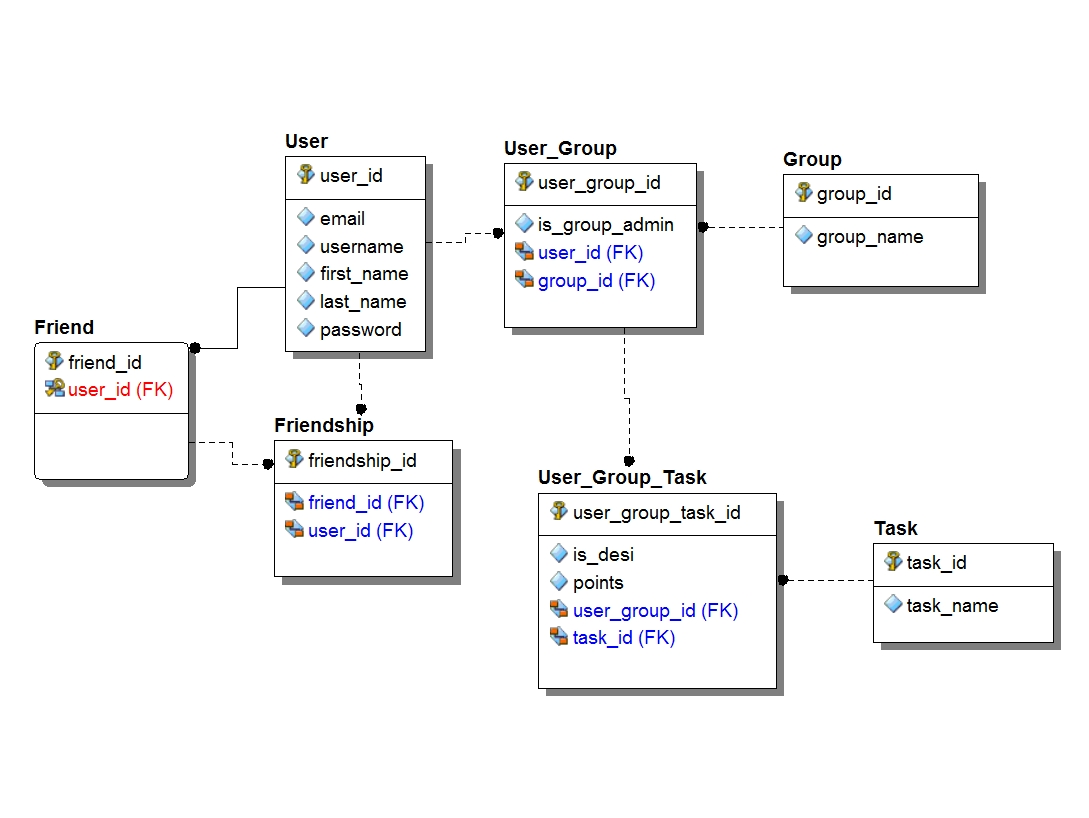
\includegraphics[scale=0.5]{desiErd.png}

\section{Conceptual Model of the Enterprise}
\begin{table}[H]
\centering
\caption{User Entity}
\label{}
\begin{tabular}{|l|l|}
\hline
\multicolumn{2}{|c|}{{\ul \textbf{User}}} \\ \hline
user\_id & PK, CK \\
username & CK \\
password &  \\
first\_name &  \\
last\_name &  \\
email & CK 
\end{tabular}
\end{table}

\begin{table}[H]
\centering
\caption{Group Entity}
\label{}
\begin{tabular}{|l|l|}
\hline
\multicolumn{2}{|c|}{{\ul \textbf{Group}}} \\ \hline
group\_id & PK, CK \\
group\_name &  \\
\end{tabular}
\end{table}

\begin{table}[H]
\centering
\caption{Task Entity}
\label{}
\begin{tabular}{|l|l|}
\hline
\multicolumn{2}{|c|}{{\ul \textbf{Task}}} \\ \hline
task\_id & PK, CK \\
task\_name &  \\

\end{tabular}
\end{table}

\begin{table}[H]
\centering
\caption{User\_Group Entity}
\label{}
\begin{tabular}{|l|l|}
\hline
\multicolumn{2}{|c|}{{\ul \textbf{User\_Group}}} \\ \hline
user\_group\_id & PK, CK \\
user\_id & FK references user.user\_id \\
group\_id & FK references group.group\_id \\
is\_group\_admin & 
\end{tabular}
\end{table}

\begin{table}[H]
\centering
\caption{User\_Group\_Task Entity}
\label{}
\begin{tabular}{|l|l|}
\hline
\multicolumn{2}{|c|}{{\ul \textbf{User\_Group\_Task}}} \\ \hline
user\_group\_task\_id & PK, CK \\
user\_group\_id & FK references user\_group.user\_group\_id \\
task\_id & FK references task.task\_id \\
is\_desi &  \\
points & 
\end{tabular}
\end{table}

\begin{table}[H]
\centering
\caption{Friendship Entity}
\label{}
\begin{tabular}{|l|l|}
\hline
\multicolumn{2}{|c|}{{\ul \textbf{Friendship}}} \\ \hline
friendship\_id & PK, CK \\
user\_id & FK references user.user\_id \\
user1\_id & FK references user.user\_id
\end{tabular}
\end{table}


\section{Table Dictionary}
\begin{table}[H]
\centering
\begin{tabular}{|l|l|l|}
\hline
\multicolumn{1}{|c|}{{\ul \textbf{Table}}} & {\ul \textbf{Attributes}} & {\ul \textbf{Description}} \\ \hline
User & \begin{tabular}[c]{@{}l@{}}user\_id (PK),\\ username, \\ first\_name,\\ last\_name, \\ password \end{tabular} & A user of the application. \\ \hline
Friendship & \begin{tabular}[c]{@{}l@{}} friendship\_id(PK), \\ user\_id (FK), user\_id1 (FK) \end{tabular} &A friendship between 2 users of the application. \\ \hline
Group & \begin{tabular}[c]{@{}l@{}}group\_id (PK), \\ group\_name \end{tabular} & A group of users that contains tasks. \\ \hline
Task & \begin{tabular}[c]{@{}l@{}}task\_id (PK),\\ task\_name \end{tabular} & \begin{tabular}[c]{@{}l@{}}A task to be completed by \\ a given user in a group.\end{tabular} \\ \hline
User\_Group & \begin{tabular}[c]{@{}l@{}}user\_group\_id (PK), \\ user\_id (FK),\\ group\_id (FK), \\ is\_group\_admin\end{tabular} & Relationship between users and groups. \\ \hline
User\_Group\_Task & \begin{tabular}[c]{@{}l@{}}user\_group\_task\_id (PK), \\ user\_group\_id (FK), \\ task\_id (FK),\\ is\_desi, \\points\end{tabular} & \begin{tabular}[c]{@{}l@{}}Relationship between usergroups and\\ tasks.\end{tabular} \\ \hline
Group & \begin{tabular}[c]{@{}l@{}}friendship\_id (PK), \\ user\_id (FK), \\ friend\_id (FK) \end{tabular} & Relationship between two users. \\ \hline
Task\_Action & \begin{tabular}[c]{@{}l@{}}task\_action\_id (PK), \\ user\_group\_task\_id (FK) \end{tabular} & The act within a task. \\ \hline
Completion & \begin{tabular}[c]{@{}l@{}}task\_action\_id (FK), \\ completion\_time \end{tabular} & The completion a task by the desi. \\ \hline
Volunteer\_Completion & \begin{tabular}[c]{@{}l@{}}task\_action\_id (FK), \\ volunteer\_completed \end{tabular} & The completion a task by a volunteer. \\ \hline
\end{tabular}
\end{table}

\section{Attribute Dictionary}
\begin{table}[H]
\centering
\begin{tabular}{|l|l|l|}
\hline
\multicolumn{1}{|c|}{{\ul \textbf{Attribute}}} & {\ul \textbf{Description}} & {\ul \textbf{Tables Found In}} \\ \hline
user\_id & Primary key for users & \begin{tabular}[c]{@{}l@{}}User, User\_Group (FK),\\ Friendship (FK)\end{tabular} \\ \hline
username & Unique identifier of a user & User \\ \hline
first\_name & The first name of a user. & User \\ \hline
last\_name & The last name of a user. & User \\ \hline
password & The password of a user. & User \\ \hline
email\_address & The email of a user. & User \\ \hline

group\_id & Primary key for groups. & \begin{tabular}[c]{@{}l@{}}Group, User\_Group (FK),\\ User\_Group\_Task (FK)\end{tabular} \\ \hline
group\_name & The name of a group. & Group \\ \hline
is\_group\_admin & \begin{tabular}[c]{@{}l@{}}Boolean that says whether a\\ user is a group admin.\end{tabular} & User\_Group \\ \hline

user\_group\_id & Primary key for a user\_group. & \begin{tabular}[c]{@{}l@{}}User\_Group,\\ User\_Group\_Task (FK)\end{tabular} \\ \hline

user\_group\_task\_id & \begin{tabular}[c]{@{}l@{}}Primary key for a\\ user\_group\_task.\end{tabular} & User\_Group\_Task \\ \hline
points & \begin{tabular}[c]{@{}l@{}}Number of points a user has\\ for a given task.\end{tabular} & User\_Group\_Task \\ \hline
is\_desi & \begin{tabular}[c]{@{}l@{}}Boolean that say whether a\\ user is the person responsible\\ for completing a given task.\end{tabular} & User\_Group\_Task \\ \hline

task\_name & The name of a task. & Task \\ \hline
task\_id & The primary key of a task. & \begin{tabular}[c]{@{}l@{}}Task,\\ User\_Group\_Task (FK)\end{tabular} \\ \hline

friendship\_id & Primary key of a friendship. & Friendship \\ \hline

\end{tabular}
\end{table}


\chapter{Database and Query Definition}
\section{Database Definition}
\lstinputlisting[language=SQL, breaklines=true]{desi_create.sql}

\section{English version of 10+ database queries, and the SQL DML for each query}
\subsection{English version}
\begin{enumerate}
\item How many users are in the group with group.id = 2?
\item Who is the desi for task \"Empty Dishwasher\" in the group with group.id = 1?
\item How many groups is user with username \"mwflickner\" in?
\item How many points does user \"mwflickner\" have in task "Take Out Trash" in group with group.id = 1?
\item When was the last time the task "Empty Dishwasher" in group with group.id = 1 completed?
\item What is the first name and the last name of the user with user.id = 2?
\item How many points does user with user.user\_id = 1 have among all of his tasks in group with group.id = 3?
\item How many points does user with user.user\_id = 1 have among all of his tasks in all of his groups?
\item How many points are there total in this application?
\item Who are the users who have performed an opt out? 
\end{enumerate}

\subsection{SQL DML}
\lstinputlisting[language=SQL]{desi_10_queries.sql}


\section{Review sign-off sheet}
See attached review.

\section{Design Limitations}
One of the design limitations I ran into with Desi was being unable to track and log past actions for tasks. I revised my model and added the Task\_Action along with Task\_Completion, Volunteer\_Completion, Opt\_Out to track task actions and the types of actions. A limitation that I currently have is that points from a task are restricted to only those tasks and cannot be applied to other tasks.

\chapter{Database Integrity and Security}
\section{Functional Dependencies}
\subsection{Table: User}
user\_id $\rightarrow$ username, first\_name, last\_name, email\_address, password \\
username $\rightarrow$ user\_id, first\_name, last\_name, email\_address, password \\
email\_address $\rightarrow$ user\_id, first\_name, last\_name, email\_address, password \\

\subsection{Table: Group}
group\_id $\rightarrow$ group\_name

\subsection{Table: UserGroup}
user\_group\_id $\rightarrow$ is\_group\_admin, user\_id (FK), group\_id (FK)\\
user\_id (FK), group\_id (FK) $\rightarrow$ user\_group\_id, is\_group\_admin

\subsection{Table: UserGroupTask}
 user\_group\_task\_id $\rightarrow$ points, is\_desi, user\_group\_id (FK), task\_id (FK)\\
 user\_group\_id (FK), task\_id (FK) $\rightarrow$ user\_group\_task\_id, points, is\_desi
 
 \subsection{Table: Task}
 task\_id $\rightarrow$ task\_name
 
 \subsection{Table: Completion}
 user\_group\_task\_action\_id $\rightarrow$ completed\_date
 
 \subsection{Table: VolunteerCompletion}
 user\_group\_task\_action\_id $\rightarrow$ volunteer\_completed
 
 \subsection{Table: Opt-Out}
  user\_group\_task\_action\_id $\rightarrow$ opt\_out\_date

\section{Adjustments for Normalization}
My database design did not require any normalization adjustments as it is already normalized.

\section{Integrity and Security}
Users have the ability to write to other tables but only delete Friendships or themselves. GroupAdmins can delete anything group or task related. All emails, usernames, passwords need to be validated by a regex to make sure they fit the proper requirements.

\chapter{Implementation}
\section{Indices}
Indices will be placed on the primary keys of each table.
\section{Data}
\lstinputlisting[language=SQL, breaklines=true]{desi_sample_data.sql}
\section{Query Trace}
Unfortunately, I could not get the query trace working. However I can verify that all of the queries ran and returned the correct results.

\section{Implementation Assessment}
All in all, I thought I implemented my design very well. At first there were a lot of kinks I need to work out, but as the semester progressed I felt very confident about all of the improvements I made. The biggest key to the whole project was honestly the ERD. Once I had that, everything else was easy. Every time I had to change the ERD, I had to change pretty much everything. MySQL Workbench was incredibly helpful with the ERD and being able to generate the SQL create file from my ERD was incredibly useful.

\chapter{Lessons Learned}
\par I learned a great deal of things during this project. I obviously made some mistakes along the way but I definitely learned a lot of things and if I had to do this project again, I would go about it a lot differently. First of all, if I were to do this project again, the first thing I would do would be the ERD. The ERD was the core of the entire project and doing other things differently before that was pointless because if I changed one little thing about the ERD I would have to go back and redo all of the sections I previously did. It turned into a big waste of time doing that and I didn't get much out of it. Rather, next time I would do the ERD first and get it right. Once I got the ERD right I would proceed to the other steps.
\\
\par The next thing I learned was that \LaTeX is the way to go. I initially started doing this project in Microsoft Word and let me tell you, it was terrible. Using \LaTeX cleaned up my project so much and made it much easier to do all of the write-ups. I was also much more organized when I used it. The \LaTeX packages were also super useful when it came to building tables and getting them to look the way I wanted them too. I highly recommend using an online \LaTeX table generator as well because it made life so much easier.
\\ 
\par Next up was ER Studio and MySQL Workbench. Honestly, if i had to do the project again, I would scrap ER Studio and just use mySQL Workbench. The software seemed old and outdated and the user interface was very confusing. MySQL Workbench had a cleaner user interface and had better documentation online as far as how to user the software. It was very easy to generate both a create script in SQL and then a populate script. I would highly recommend MySQL Workbench.
\\
\par I am not exactly sure how many hours I spent on the project but if I had guess I would say it would be around 45 total hours. Dividing that up it comes to around 3.5 hours a week. But a lot of that was clustered around the due dates of the deliverables. And there wasn't always a deliverable every week. Honestly, a lot of the time spend was going back and redoing work that I had already done, which as I mentioned earlier could have been avoided if the ERD had been completed first.
\\
\par The project definitely taught me how to write and read SQL a lot better. It also taught me when I should actually write SQL and when I could not. For example I should not write the SQL create script for my database, rather I should let MySQL Workbench generate it from my ERD and then from there just write my queries. The project also helped me really understand functional dependency and normalization a lot better. Using MySQL was definitely the best call over other options. PHPmyAdmin was pretty cool as well, I liked having such a visual way of interacting with my database.

\end{document}